Los criterios a evaluar fueron estimados con el rango de notas de 1 a 7, sacando un promedio de cada integrante del equipo según la percepción que obtuvo al utilizar el software: \\

\begin{center}
\begin{tabular}{|l|c|p{2.40in}|}
 \hline
 \textbf{Criterio} & \textbf{Nota} & \textbf{Comentario} \\
 \hline
 \textbf{Fácil de Implementar} & 7.0 & Es una herramienta 100\% web, por lo que no necesariamente el software necesita ser instalado en el computador. \\
 \hline
 \textbf{Facilidad de uso} & 5.0 & Presenta una interfaz poco intuitiva (Diseño Drag and Drop). \\
 \hline
 \textbf{Estándares} & 6.0 & No utiliza la misma notación de BPMN 2.0 pero son semejantes, su notación esta orientada a SOA (arquitectura orientada a servicios). \\
 \hline
 \textbf{Licencia} & 7.0 & ProcessMaker brinda a las organizaciones las ventajas de open source. \\
 \hline
 \textbf{Documentación y Soporte} & 7.0 & La página web del software presenta una gran variedad de documentación , vídeos y foros en que se enseña a utilizar el software, además posee un servicio de soporte. \\
 \hline
\end{tabular}
\end{center}

\subsection{Ejemplo de Proceso de obtención de tarjeta de crédito}
Para la utilización del software ProcessMaker, según el modelamiento de procesos, se utilizó como referencia un video de youtube que explicaba la obtención de una tarjeta de crédito en un banco.

También se pudo observar que este software posee la capacidad de que el administrador pueda interactuar con cualquier trabajador de la empresa en algún proceso, puesto que existe la opción de agregar usuarios, grupos o departamentos, en que el administrador puede asignarles tareas o sub-tareas, también poder enviarles reportes, mensajes (en el mismo software hay un inbox) o mails. Además esta la opción que si alguna tarea requiere de la creación de formularios, se realiza de forma dinámica, en el ejemplo de la tarjeta de crédito se requiere en la tarea de ``Rellenar Solicitud", un formulario en que se ingresen los datos del cliente y fecha en que se realizó la solicitud, entonces en esta tarea el usuario de la empresa asignado en esta tarea tendrá la misión de ingresar mediante este formulario los clientes que serán luego guardados en una base de datos del mismo software.
 
\begin{center}
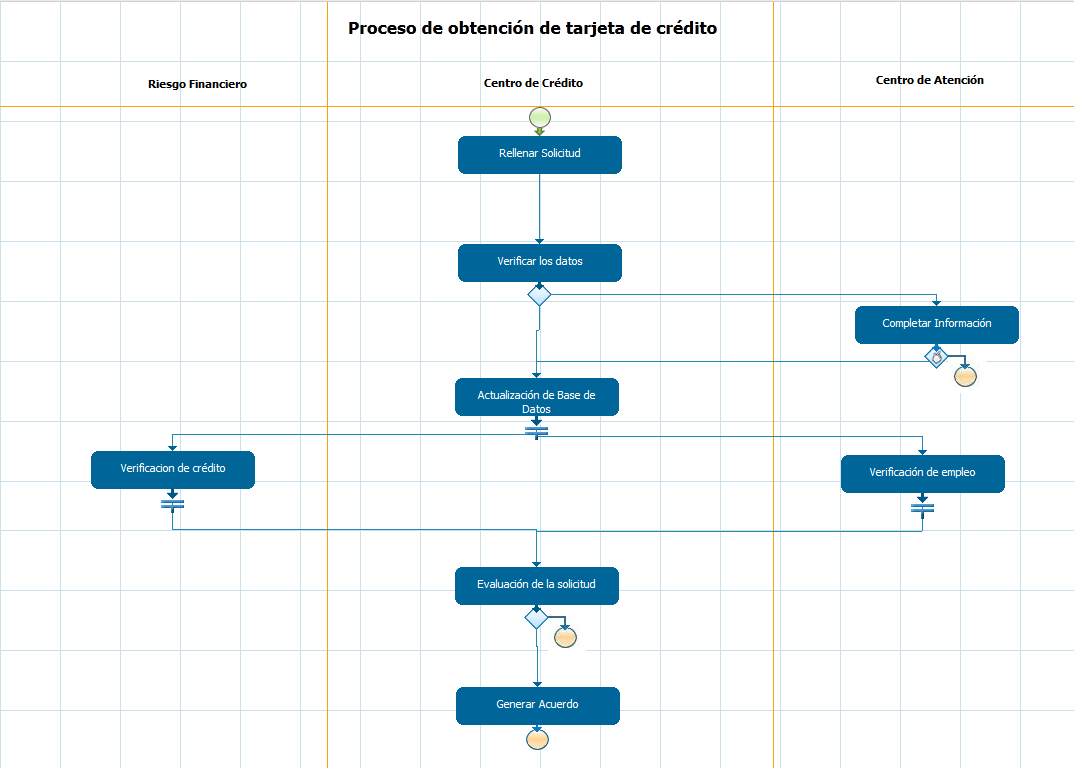
\includegraphics[scale=0.5]{./imagenes/modelos_pm.png}\\
     Figura 1: Modelo en Process Maker.\\
\end{center}

A continuación se muestra la notación del software:

%ingresar la notación
Para añadir elementos al diagrama:

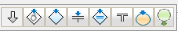
\includegraphics[scale=0.8]{./imagenes/menu.png}

Estas herramientras permiten dibujar el flujo de los procesos a dibujar.
Luego de añadir los elementos al mapa de procesos, hacer clic derecho en cualquier lugar en un área en blanco del mapa y selecciones una opción desde el siguiente menú.

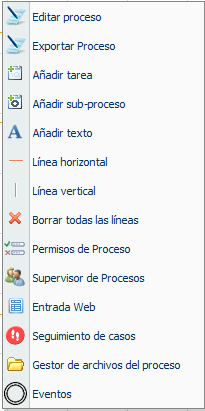
\includegraphics[scale=0.8]{./imagenes/clickmenu.png}

\begin{itemize}
\item  Editar Procesos: Esta opción permite tanto al nombre del proceso como a su descripción ser modificados. También provee opciones para activar Modo de Depuración y establecer un calendario para el proceso.
\item Exportar proceso: Un Proceso puede ser exportado para ser usado en una instalación de ProcessMaker. Para más información, ver Importar y Exportar Procesos.
\item Añadir Tarea: Añade una nueva tarea al mapa de procesos.
Añadir un SubProceso: Sub-procesos permite a los casos ejectutados como subprocesos dentro de procesos maestros.
\item Añadir Texto : Las etiquetas de texto adicional pueden estar añadidas al mapa de procesos. Este texto puede ser usado para etiquetar un grupo de tareas, identificar departamentos en la organización, explicar la lógica de ruta, o incluso de proveer una guía al usuario.

\item Linea Horizontal : Añade una línea horizontal al Mapa de Procesos, para ayudar a visualizar y dividir los proceso. Las líneas suelen ser usadas para separar tareas o departamentos de su organización en una agrupación lógica en su mapa de Procesos.

\item Linea vertical: Añade una línea vertical al Mapa de Procesos, para ayudar a visualizar y dividir el proceso. Las líneas pueden ser usadas para separar tareas o departamentos de su organización en agrupaciones lógicas en su mapa de procesos.

\item Eliminar todas las líneas: Esta opción eliminará todas las líneas horizontales y verticales en el mapa de procesos.

\item Permisos de Proceso: Use Permisos de Procesos para dar a los usuarios específicos acceso de sólo lectura a la información acerca de los casos. (Para escribir acceso a los casos, ver Supervisor de Procesos.) Los Permiso de Procesos pueden ser definidos, así que los usuarios específicos pueden ver o no objetos específicos en casos, como en DynaForms, Documentos de entrada y Documentos de Entrada.

\item Supervisor de Procesos: Supervisor de Procesos esta designado a usuarios que pueden acceder a los casos desde los procesos y cambiar los datos de un caso en DynaForms y Documentos de Entrada, sin estar asignados a una tarea en particular en el proceso. Use este sub menú para especificar a qué objetos del supervisor de Procesos se puede acceder.

\item Entrada Web: Entrada Web es una opción para iniciar nuevos casos desde una DynaForm desplegado en una página web externa.

\item Seguimiento de Casos: El Seguimiento de Casos permite a los usuarios externos a seguir el progreso de un caso y acceder a la información acerca de ese caso a través de un código de caso y un PIN. Use este sub menú para especificar a qué objetos tiene permiso para ver el usuario externo con Seguimiento de Casos.

\item Administrador de Archivos de : Use el Administrador de Archivos de Procesos para cargar un documento externo en ProcessMaker. De manera distinta a los archivos de Documentos de entrada, que usualmente cambian para cada nuevo caso, esta opción es usada generalmente para archivos que son ineditables y son requeridos por todos los casos en un proceso. El Administrador de Archivos de Procesos puede también crear plantillas de correo que usualmente son usadas para enviar Notificaciones.

\item Eventos: Eventos Permite a un trigger ser activado o a un correo electrónico ser enviado en un momento específico durante un proceso.
\item Tips para el uso del Mapa de Procesos:
Debido a que ProcessMaker es una aplicación web-based, ocasionalmente puede tener problemas para salir de los cuadros de diálogo en el Mapa de Procesos. Si ProcessMaker se cuelga cuando se despliega un cuadro de diálogo, retorne al proceso principal haciendo clic en el Mapa de Procesos haciendo clic en el 
File:RefreshBotón.png Actualizar del buscador Web.
El Mapa de Procesos no ofrece una opción de des hacer y no permite guardar diferentes versiones del mapa. Si usted se anticipa a experimentar con el mapa, puede ser posible que quiera retornar a una versión previa del mapa después de hacerlo, por ello recomendamos exportar el proceso antes de hacer algún cambio. Para volver a una versión previa del mapa, elimine o re nombre el proceso en curso en importe la versión previa.

\end{itemize}